\documentclass[a4paper]{article}
\usepackage{fancyhdr} % Required to make the custom header and footer
\usepackage{lastpage} % Required to determine the last page for the footer
\usepackage{ stmaryrd }
\usepackage{ amssymb }
\usepackage{listings}
\usepackage{graphicx}
\usepackage{systeme}
\usepackage{wrapfig}

%%%%%%%%%% MODIFY THE FOLLOWING WITH YOUR INFORMATION %%%%%%%%%%

%Names of students (If only one, put a '~' as the second name
\newcommand{\firstStudent}{Alessandro Romanelli}
\newcommand{\secondStudent}{Edoardo Lunardi}

%Subject's name
\newcommand{\subjectName}{Programming Fundamentals 1}
%Current semester (Fall/Spring + Year)
\newcommand{\semester}{Fall 2017}
%Date (put '\today' for current date)
\newcommand{\theDate}{\today}
%Title of the document (i.e. Assignment 1)
\title{\Huge Project Presentation}
%%%%%%%%%%%%%%%%%%%%%% END %%%%%%%%%%%%%%%%%%%%%%%



%\usepackage{showframe}

%---------------------- Custom Commands ----------------------
\newcommand{\question}[1]{
\section*{Question #1 }
}

\newcommand*{\QEDA}{\hfill\ensuremath{\blacksquare}}%
\newcommand*{\QEDB}{\hfill\ensuremath{\square}}%

%---------------------- Layout Setup ----------------------
%Names
\fancyhead[L]{\firstStudent\\\secondStudent}
%Subject name
\fancyhead[C]{\semester\\\subjectName}
%Date (Leave as is for today's date)
\fancyhead[R]{\theDate\\USI Lugano}
% Footer
\fancyfoot[C]{Page\ \thepage\ of\ \pageref{LastPage}}
%Height of the line separating Header and main content
\renewcommand{\headrulewidth}{0.5pt}
\renewcommand{\footrulewidth}{0.5pt}
%Hide the date from the maketitle command
\date{}
\author{by Alessandro Romanelli \& Edoardo Lunardi}
%Custom margins
\usepackage[margin=35mm]{geometry}


\pagestyle{fancy}
\makeatletter
\def\@maketitle{%
  \newpage
  \vspace*{\fill}      % remove the initial space
  \begingroup\centering    % instead of \begin{center}
  \let \footnote \thanks
  \hrule height \z@        % to avoid the insertion of lineskip glue
    {\Huge \@title \par}%
    \vskip 0em
    {\large
      \lineskip 0em
      \begin{tabular}[t]{c}%
        \@author
      \end{tabular}\par}%
    \vskip 1em
    {\large \@date}%
  \par\endgroup            % instead of \end{center}
  \vskip 1.5em             % <--- modify this to adjust the separation
  \vspace*{\fill}
}
\let\ps@plain\ps@fancy
\makeatother

\begin{document}
\maketitle
\begin{figure}[b]
  \centering{
\includegraphics[width=0.8\textwidth]{USI_logo_2.png}}
\end{figure}
\newpage
\tableofcontents %the table of contents is automatic
\newpage

\section{Introduction}
\paragraph{} Welcome to the presentation of this project by \textbf{Alessandro Romanelli} and
\textbf{Edoardo Lunardi}. We have been a team for the whole course and decided to stick together
also for the final milestone of this semester. \par

\section{Intention}
\paragraph{} We want to create a \emph{Vertical Scroller Game}, that is a game where the player has to fight through some obstacles whilst navigating towards the top of the screen. The further up the player is able to go, the more points he obtains. The goal of the game should be to achieve the most points possible before dying.

\section{Goals}
In this section we are going to discuss our main objectives for this project.
\subsection{Minimal Valuable Product}
 Our basic game should consist of the following features upon submitting the project for the final deadline:
 \begin{itemize}
   \item The player should be able to move along the X-Axis alone;
   \item Player will shoot throughout the whole game;
   \item Walls consisting of $n$ number of blocks should be scrolling down towards the player;
   \item Each block should have health points;
   \item When a block has 0HP it should disappear;
   \item Upon contact between a block and the player, the game should end;
   \item Player's score should be evaluated constantly based on damage dealt;
   \item Score will always be visible to the player whilst playing.
 \end{itemize}
 \newpage
\subsection{Extra Features}
We also thought about expanding the project if we are early on our submission by implementing the following aspects to our base project:
\begin{itemize}
  \item Blocks' health should be randomly generated and not hardcoded;
  \item Blocks should change color depending on the their HP;
  \item Time elapsed should have an effect on difficulty (the more time passes, the harder the game gets);
  \item Power ups should be randomly spawned to help the player
  \begin{itemize}
    \item Immunity for $n$ seconds;
    \item Firing speed increased;
    \item Volley fire, three or more trajectories;
    \item Next shot is a one-hit kill;
  \end{itemize}
  \item Special Attack with cooldown to destroy the entire wall, without yielding points;
  \item Special properties for some random walls' blocks:
  \begin{itemize}
    \item Blocks that reflect the player fire;
    \item Undestroyable blocks;
    \item For each HP, a special block yields twice the points;
  \end{itemize}
  \item The game should be able to remember and store the highest score of the player, in order to remember it when restarting the program.
  \item At the end of the game, player should be prompted to insert name for record;
  \item Implement a game menu, where player can either:
  \begin{itemize}
    \item Start a new game;
    \item Quit the game;
    \item View the leaderboard
  \end{itemize}
  \item Store the game leaderboard into a file that can be accessed upon restarting the game to save progression.
\end{itemize}
\newpage
\subsection{Sketch}
\begin{figure}[h]
  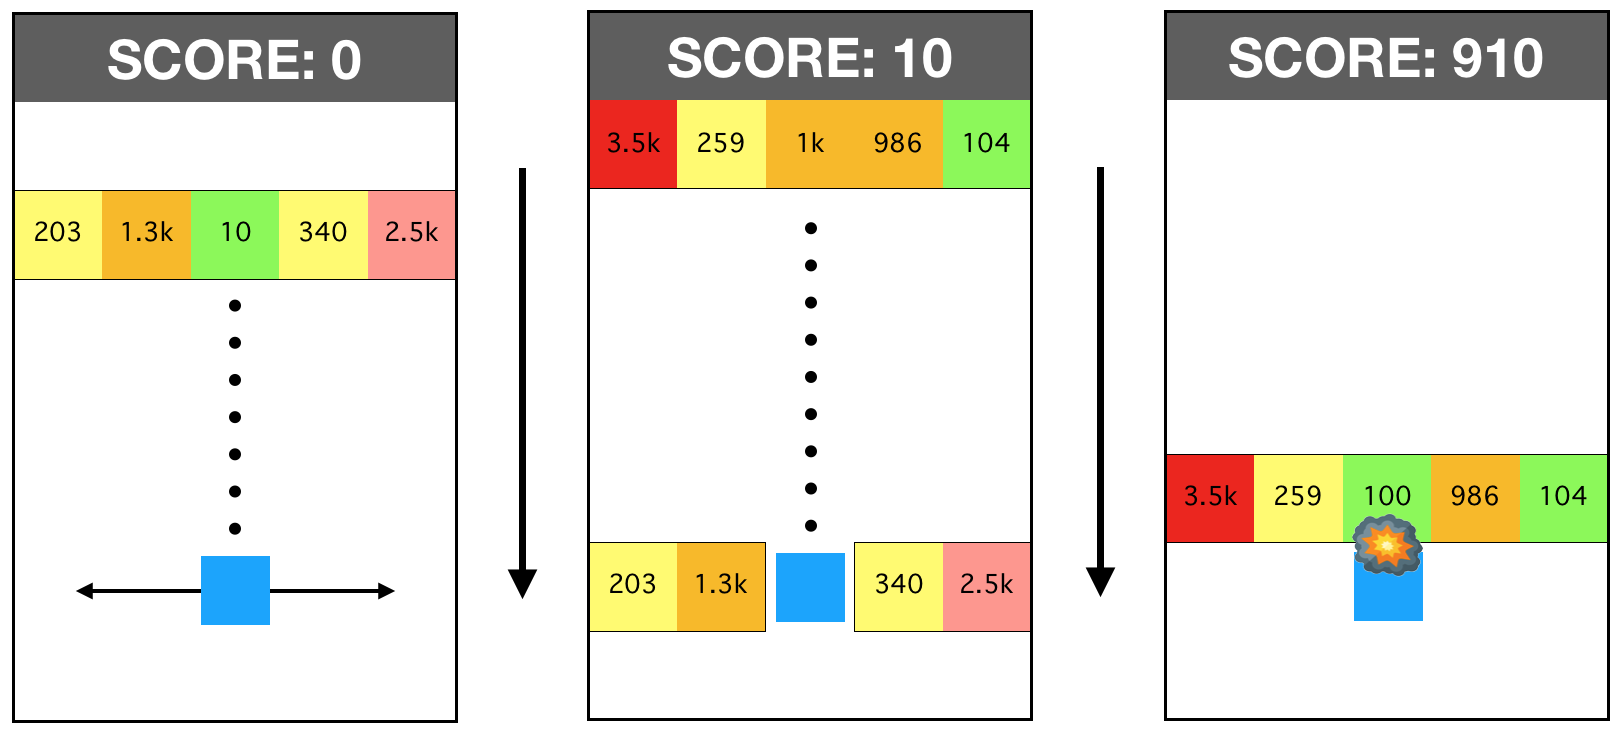
\includegraphics[width=\textwidth]{sketch.png}
  \caption{A very simplified sketch idea of the basic game}
\end{figure}

\section{Execution}
\paragraph{} Our first efforts are going to go towards the development of \textbf{MVP}, which we are pretty sure to be achievable by using the \emph{Racket Language}. \\ \\
However, we are going to use our most familiar libraries that are \texttt{2htdp/image} for the sprites and \texttt{2htdp/universe} for the big-bang application. \\ \\ In order to implement some of extra features that we spoke about in the previous sections we might also conduct a more extensive research if need be, but we are pretty sure that the project is doable with what stated previously.

\section{Logistics}
\subsection{Methods}
  \paragraph{} In order to develop and deploy our project we are going to use a \emph{Git} version control system to keep our files in check and allow us to develop our program simultaneously and avoid us any pain with conflicts.
\subsection{Location}
  \paragraph{} We are going to host our code publicly on \emph{GitHub} at this address: \\ https://github.com/AlessandroRomanelli/pf1-project.git

\section{Conclusion}
\paragraph{} We are most happy to begin working on our project and deliver a videogame that is replayable, most fun and addictive as possible!


\end{document}
